\chapter{Conceptos clave} % Main appendix title
\label{appendix:keyconcepts} % For referencing this appendix elsewhere, use \ref{AppendixA}

La mayor parte de este apéndice se basa en contenido expuesto en \cite{deeplearning}.

\section{Estimadores, Parcialidad (\glsentrylong{bias}) y Varianza}
% \todo[inline]{Por hacer, pagina 119 Deep Learning}
El campo de las estadísticas nos da muchas herramientas para conseguir nuestro objetivo de \gls{machinel} de resolver una tarea no solo con el conjunto de entrenamiento sino que también para generalizar. Conceptos fundamentales como la estimación de puntos, la parcialidad y la varianza son útiles para caracterizar formalmente las nociones de generalidad, \gls{underfitting} y \gls{overfitting}.

\subsection{Estimación de puntos}
La estimación de puntos es el intento de proveer la única ``mejor'' predicción de alguna cantidad de interés. En general esta cantidad de interés puede ser un único parámetro o un vector de parámetros en algún modelo perimétrico.

Para distinguir estimados de parámetros de su valor real se utiliza la distinción de un parámetro $\vtheta$ con $\hat{\vtheta}$.

Sea $\{ \vx^{(1)}, \ldots, \vx^{(m)} \}$ un conjunto de $m$ puntos de datos independiente e idénticamente distribuidos. Un \textbf{estimador} o \textbf{estadístico} es cualquier función en base a los datos:
\begin{equation}
  \hat{\vtheta}_m = g( \vx^{(1)}, \ldots, \vx^{(m)} )
\end{equation}

Sin embargo, la definición no requiere que $g$ sea una buena estimación del verdadero $\vtheta$ ni tampoco que la respuesta este en el mismo conjunto de valores validos de $\vtheta$. Esta definición supone una gran flexibilidad para definir un estimador, sin embargo un buen estimador es una función cuya salida sea cercana al verdadero $\vtheta$ que genero los datos de entrenamiento.

Podemos asumir (desde la perspectiva de frecuentista) que el valor verdadero del parámetro $\vtheta$ es fijo pero desconocido, y que $\hat{\vtheta}$ es una estimación en función a los datos.

\subsubsection{Estimación de funciones}
La estimación de puntos también puede hacer referencia a la estimación de la relación entre variables entrada y objetivo, nos referimos a estos tipos de estimación de puntos como estimación de funciones.

En este escenario tratamos de predecir una variable $\vy$ dado un vector de entrada $\vx$. Asumimos que existe una función $f(\vx)$ que describe una relación aproximada entre $\vy$ con $\vx$. Podemos asumir que $\vy = f(\vx) + \vepsilon$, donde $\vepsilon$ es la parte de $\vy$ que no es predecible a partir de $\vx$. En la estimación de funciones nos interesa aproximar $f$ con un modelo o estimado $\hat{f}$.

\subsection{Parcialidad (\glsentrylong{bias})}
La parcialidad (o \gls{bias} en inglés) es un estimador definido como:
\begin{equation}
  \mathrm{bias}(\hat{\vtheta}_m) = \E(\hat{\vtheta}_m) - \vtheta
\end{equation}

Donde la el valor esperado es sobre los datos (vistos como muestras de una variable aleatoria), donde $\vtheta$ es el valor verdadero de $\vtheta$ usado para definir la distribución que generadora de los datos. Un estimador se dice que es imparcial (o \textsl{unbiased} en inglés) si $\mathrm{bias}(\hat{\vtheta}_m) = \vzero$, lo cual implica que $\E(\hat{\vtheta}_m) = \vtheta$. Un estimador se dice que es \textbf{asintótico imparcial} si $\lim_{m\to\infty}\mathrm{bias}(\hat{\vtheta}_m) = \vzero$.

Los estimadores imparciales son ciertamente deseables, sin embargo no son siempre los ``mejores'' estimadores.

\subsection{Varianza y Error Estándar}
Otra propiedad de un estimador que puede que debamos tener en cuenta es que tanto se espera que van a variar nuestros resultados como función de la muestra de datos.

La \textbf{varianza} de un estimador se define como:
\begin{equation}
  \Var(\hat{\rvtheta})
\end{equation}

donde la variable aleatoria $\hat{\rvtheta}$ es el conjunto de entrenamiento. De manera alternativa la raíz cuadrada de la varianza es el \textbf{error estándar}, denotado como $\standarderror(\hat{\rvtheta})$.

La varianza (o el error estándar) de un estimador nos provee de una medida de como esperaríamos que el estimado que computamos de los datos variara cuando retomamos una muestra independiente del conjunto de datos. De la misma manera en que nosotros querríamos una parcialidad baja, querríamos también una varianza baja.

El error estándar de la media esta dado por:
\begin{equation}
  \standarderror(\hat{\mu}_m) = \sqrt{ \Var{\Bigg[ \frac{1}{m} \sum_{i=1}^{m} x^{(i)} \Bigg]} } = \frac{\sigma}{\sqrt{m}}
\end{equation}
    
La varianza de un estimador disminuye en función de $m$, el numero de muestras de nuestro conjunto de datos.

\subsection{Consistencia}
En la labor de escoger un mejor estimador nos interesa especialmente como este se comportara a medida que la cantidad de datos de entrenamiento aumenta. En particular nos interesa que a medida que la cantidad de datos aumenta nuestros estimados se aproximan cada vez mas al verdadero valor de los parámetros. Formalmente deseamos:

\begin{equation} \label{eq:consistency}
  \plim_{m\to\infty} \hat{\rvtheta} = \rvtheta
\end{equation}

El símbolo $\plim$ indica convergencia en probabilidad, indicando que para cualquier $\epsilon > 0$ se tiene que $P(|\hat{\rvtheta} - \rvtheta| > \epsilon) \to 0$ cuando $m \to \infty$. La condición descrita en la \equationref{eq:consistency} se le conoce como \textbf{consistencia}.

La consistencia nos asegura que la parcialidad inducida por el estimador se elimina a medida que la cantidad de muestras de datos aumenta. Sin embargo lo contrario no es verdad --- imparcialidad asintótica no implica consistencia.

A medida que la capacidad del modelo aumenta, la parcialidad tiende a disminuir y la varianza tiende a aumentar, dándonos así una curva en forma de U para el error de generalización, tal como se muestra en la \figureref{fig:consistency}.

\begin{figure}[H]
  \centering
  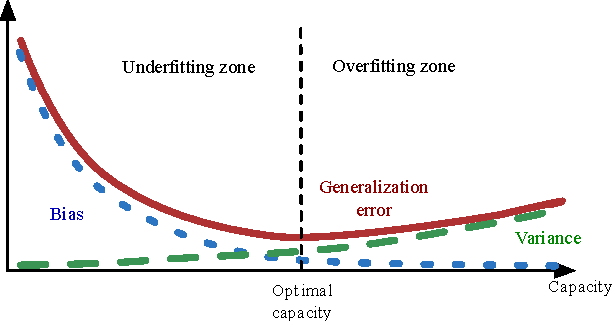
\includegraphics[width=0.7\textwidth]{Figures/consistency.pdf}
  \decoRule
  \caption[Consistencia]{Consistencia. Tomado de \cite{deeplearning}.}
  \label{fig:consistency}
\end{figure}

\section{Capacidad, \glsentrylong{overfitting} y \glsentrylong{underfitting}}
\todo[inline]{Por hacer, pagina 107 Deep Learning}

\subsection{Regularización}
\todo[inline]{Por hacer}

\section{Hiper-parámetros y conjuntos de Validación}
\todo[inline]{Por hacer, pagina 117 Deep Learning}

\subsection{Validación cruzada}
\todo[inline]{Por hacer}

\section{Curva \glsentryname{roc} y valor \glsentryname{auc}}
\todo[inline]{Por hacer, usar \cite{Zou2007}, esto se necesitara para los resultados de los experimentos}
\gls{roc} y \gls{auc}
